% this file is called up by thesis.tex
% content in this file will be fed into the main document
\ifpdf
    \graphicspath{{2/figures/PNG/}{2/figures/PDF/}{2/figures/}}
\else
    \graphicspath{{2/figures/EPS/}{2/figures/}}
\fi
\chapter{Related works} % top level followed by section, subsection
\label{Chap2}
Both the SVM and boosting-based learning algorithms, and their applications to various tasks in image processing are extremely widespread. In this chapter we outline the works most closely related to the presented methods, since the size constraints of the paper do not allow for a detailed review of this area. 
% ----------------------- contents from here ------------------------
\section{Overview}
In general, classification is a problem of identifying to which set, or category belongs the next observation. The categories may be given beforehand, or derived from the data itself by application of a chosen clustering method. Usually, a certain set of data samples is given beforehand (training dataset), which serves as a basis by which the membership of the new sample is determined. The data samples are transformed into a set of explanatory variables, or features, and from them the category-defining model, or classifier, is built.

While the distinction between offline and online algorithms for training classifiers is not clearly defined, it is usually accepted that the offline systems have random access to all training data at the same time, and that the model resulting from this data should asymptotically converge to the equilibrium. In this setting, the training time is less important.  On the other hand, online systems have only limited access to the data, usuallly to a single sample at a time, or a few consecutive samples, and it is preferrable for the learning iteration to run in the real time, i.e. that the update iteration should take less time then the acquisition of the next data sample. 

There are several types of classifiers, such as binary or multiclass, linear, nonlinear and categorical, etc. In this paper, we focus on the linear binary classifiers, which can be used for nonlinear classification by transforming feature space. 
\section{Offline classification algorithms}

\subsection{Support vector machines}
\begin{figure}[t]
		\centering
		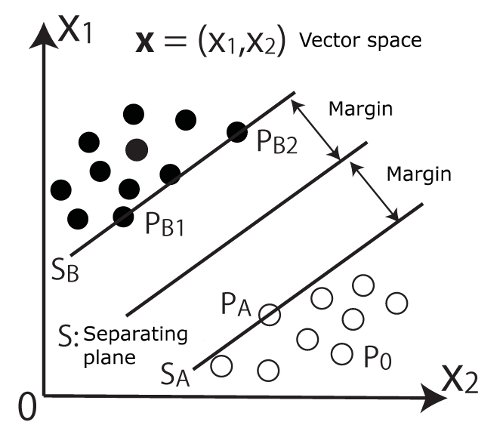
\includegraphics[width=0.5\textwidth]{margin_sep_lr}
		\caption[Maximum margin separation]{Two classes separated by a maximum margin hyperplane}
		\label{Margin}
	\end{figure}
The support vector machines are a class of linear  binary classifiers that attempt to maximize the minimal distance (margin) between classes, i.e. to construct a hyperplane in the feature space that separates the two classes and is located, intuitively, exactly in the "middle" between them (see \figref{Margin}). The mathematical formulation for this problem is: given a set of training samples $\vec{x}_i$ and associated labels $y_i$, $i\in [1..n]$, minimize in$\vec{w},b$ $\frac{1}{2}||\vec{w}||^2$ subject to $y_i(\vec{w}\vec{x}_i-b)\ge 1$. Introducing Lagrangian multiplers $\alpha_i$, the primal formulation then becomes as follows: 
\begin{equation}
\label{simplePrimal}
\min_{\vec{w},b} \max_{\alpha_i}\left\{ \frac{1}{2}||\vec{w}||^2 -\sum_{i=1}^{n}\alpha_i(y_i(\vec{w}\vec{x}_i-b)-1)\right\}
\end{equation}
The classifier output is then the sign of the confidence function $f(\vec{x},\vec{w})=\vec{w}*\vec{x}-b$,
$$
\label{ClassifierOutput}
H(\vec{x})=sign(f(\vec{x},\vec{w}))
$$

The dual formulation of the above problem 
\begin{equation}
\label{simpleDual}
\max_{\alpha_i}\left ( \sum_{i=1}^{n}\alpha_i-\frac{1}{2}\sum_{i=1}^{n}\sum{j=1}^{n}\alpha_i \alpha_j y_i y_j k(\vec{x_i},\vec{x_j})\right)
\end{equation}
subject to $\alpha_i \ge 0$,where, in original linear case, $k(\vec{x_i},\vec{x_j})=\vec{x_i}\cdot \vec{x_j}$, $\cdot$ denoting an inner product, and $\vec{w}=\sum_{i=1}^{n}\alpha_i y_i \vec{x}_i$. In this formulation, data points $\vec{x}_i$ for which $\alpha_i>0$ are called the support vectors, giving rise to the name of the method. Intuitively, these are the points that lie on the margin hyperplanes. 

Original (\cite{vapnik92}) formulation assumed that the data was linearly separable, and couldn't be solved for the noisy data. One of the most important results related to this version of classifier was that, when solvable, it was shown (\cite{Vapnik95})  to minimize the theoretical upper bound on the testing error rate. This bound is related to the VC dimension of the classifier, and  governs the relation between the capacity of a learning machine and its performance. The bound is as follows: if the classifier with parameters $\vec{\alpha}$ achieves empirical error rate, i.e. error rate on a set used for training, $R_{emp}(\vec{\alpha})$, then with probability $1-\eta$, the following bound holds: 
\begin{equation}
\label{VCbound}
R(\vec{\alpha})\le R_{emp}(\vec{\alpha})+\sqrt{\left( \frac{h(log(2l/h)+1)-log(\eta/4)}{l}\right)}
\end{equation}
where $l$ is the number of training samples and $h$ is the VC dimension of a classifier function, defined as the number maximum cardinality of a data point set that can be shattered (separated for any assignment of labels $y\in{-1;1}$ to data points). For example, a linear classifier of dimension $n$ has VC dimension of $n+1$.

SVM were then originally derived as a  family of classifiers minimizing right-hand part of \eqrefr{VCbound}, thus minimizing the expected risk and generalization error. The original classification, however, was too rigid  and not very usable on sets of data from the real world, so in \cite{SVM}, \eqrefr{simplePrimal} was rewritten,  replacing hard constraints with a loss function:

\begin{equation}
\label{expandedPrimal}
 \min_{\vec{w}} \left\{ \frac{\lambda}{2}||\vec{w}||^2 +\frac{1}{n}\sum_{i=1}^{n}l(\vec{w},(\vec{x},y)\right\}
\end{equation}
where $l(\vec{w},(\vec{x},y)$ is a loss function determining penalty for the outlier and $\lambda$ is a parameter that determines the "softness" of the margin, with large $\lambda$ favoring larger number of outliers with smaller margin.

The most commonly used loss function $l$ is a hinge-loss function, that linearly punishes the outliers and margin errors, i.e. data points that are classified correctly but lie between margin hyperplanes
$$
\label{Hingeloss}
l(\vec{w},(\vec{x},y)=\max(0, \rho-y(\vec{w}\cdot\vec{x}))
$$
where $\rho$ is a margin parameter, usually assumed to be 1 for maximum margin algorithms.

When using \eqrefr{Hingeloss}, dual form of \eqrefr{expandedPrimal} is the same as \eqrefr{simpleDual}, with the constraints changed to $0 \le \alpha_i \le C$, $C \propto \frac{1}{\lambda}$. This constrained quadratic problem is the one that is usually solved by most common offline methods.

\subsubsection{Using kernel trick to create nonlinear classifier}

It is easy to see that all of the above formulas can be expressed in terms of linear combinations of kernel function $k(\cdot,\cdot)$ on the input data samples and coefficients $\alpha_i$. For instance, confidence function of the classifier $f(\vec{x},\vec{w})=\vec{w}*\vec{x}$  can be replaced with $f(\vec{x};\{\vec{x_i},\alpha_i\,y_i\})=\sum_{i=1}^{n}\alpha_i y_i k(\vec{x},\vec{x_i})$. The linear function $k(\vec{x_i},\vec{x_j})=\vec{x_i}\cdot \vec{x_j}$ of the original formulation can then be replaced by any function satisfying Mercer's condition, i.e. any positive definite kernel. There also exists a body of research (such as \cite{negative}) that deals with practical applications of non-positive definite kernels (such as well known sigmoid function), but that lies beyond the scope of a current work. 

 The Mercer's condition, in essence, guarantees that there exists a feature space $V$, that has an operation of inner product defined in it,  and a map from the input data space $S$, $\phi : S \leftarrow V$so that kernel function between two vectors $\vec{x},\vec{y} \in S$ is equivalent to inner product: $k(\vec({x},\vec{y})=\phi(\vec{x})\cdot \phi(\vec{y})$. Essentially, the kernel trick maps input vectors $\vec{x_i}$ into larger-dimensional feature vector space $V$ , where, hopefully, the data becomes linearly separable (see {{=fig=}} for illustration).

This techniques allows using SVM as nonlinear classifier, and greatly expands the  variety of possible applications since as long as the kernel function is defined, the input vectors $\vec{x_i}$ do not even have to be numbers, and can instead be words or area descriptors in an image (\cite{bertelli2011kernelized}). However, its application also increases the costs associated with learning and using the classifier, since instead of a single vector $\vec{w}$ we have to store all nonzero $\alpha_i$ and associated $\vec{x}_i$, and the increased dimensionality of the feature space guarantees the larger possible amount of support vectors as compared to the linear formulation. Also, the same increased dimensionality increases the VC dimension of the classifier, raising bounds on the generalization error, i.e. increasing the risk of overfitting. In addition, the kernel formulation makes the primal problem much harder to solve, biasing the existing research towards quadratic dual formulation, although the methods of dealing with it exist and are introduced in  section \ref{NORMAIntro} below.
\begin{table}
\centering
    \begin{tabular}{|c|c|}
        \hline
        Kernel name                 & Function \\ \hline
        Linear                      & $\vec{x}\cdot \vec{y}$       \\ \hline
        Polynomial kernel           & $(\vec{x}\cdot \vec{y})^d$        \\ \hline
        Polynomial kernel with bias & $(\vec{x}\cdot \vec{y}+b)^d$        \\ \hline
        Gaussian RBF                & $e^{-\gamma||\vec{x}-\vec{y}||_2}$         \\  \hline
        Hyperbolic tangent          & $tanh(k\vec{x}\cdot \vec{y}+c)$        \\
        \hline
    \end{tabular}
\caption[List of SVM kernel functions]{List of the most popular SVM kernel functions}
\label{Kernels}
\end{table}
The most commonly used kernels are listed in table \ref{Kernels}.


%V. Vapnik and A. Chervonenkis. "On the uniform convergence of relative frequencies of events to their probabilities." 

\subsubsection{Common methods for offline SVM training}
Most common methods for SVM training deal with the solution to the \eqrefr{simpleDual}, and as such are usually applicable to the Quadratic Programming problems in general. Several classes of such silution techniques should be mentioned in this overview. 

{\bf Interior point methods}
IP methods (for example, \cite{boyd}) replace linear constraints of the primal with a barrier function, similar to the IP methods for linear programming.  The result is a sequence of unconstrained problems which can be optimized very efficiently using Newton or Quasi-Newton methods. The advantage of IP methods is that they achieve rapid convergence to a given accuracy bound in terms of a number of iterations. Unfortunately, they typically require run time which is cubic in the number of data samples $n$. Moreover, the memory requirements of IP  very large, so such methods are not suitable for the training sets with large number of samples.

{\bf Segmentation-based methods}
To overcome the quadratic memory requirement of IP methods, decomposition methods such as  as well-known SMO (\cite{platt}) and SVM-Light (\cite{svmlight}) work with dual variables $\alpha_i$, constrained by a set of conditions that are derived from the current state of the solution, and thus change every iteration.  In the extreme case, the active set consists of a single constraint. Therefore, the larger quadratic problem is segmented into a number of smaller ones, SMO employing the smallest subset of just two variables being optimized at a time. While algorithms of  this family are simple to implement and have general asymptotic convergence properties, the time complexity of  is  still typically super linear in the training set size $n$. 

Some of the decomposition methods can be adapted to the online learning setting, but the results are typically inferior in terms of convergence rate and accuracy to the methods specifically developed for the online setting.

{\bf Gradient-based methods}
Unconstrained gradient methods used to be common before the emergence of the more modern methods. While gradient based methods are usually known to exhibit slow convergence rates, the computational demands imposed by large scale classification problems of high dimension feature space, such as the ones common in image processing,  has revived the theoretical and applied interest in gradient methods. Many of the online methods described below, as well as our proposed algorithm, were based on the modifications of gradient methods.

\subsection{Boosting}
Boosting is a name of a family of meta-learning algorithms that boost the performance of several low- accuracy claasifiers by combining them into a single classifier with increased accuracy. Usually, a linear combination of the classifiers' outputs is used, with the goal of the corresponding algorithm being the assigment of the  weights to each classifier. In other words, given a set, or a pool of $M$ classifiers $h_i(\vec{x})$, each with error ratio $\epsilon_i$ being arbitrarily close to a result of a random classification, $0.5$,  over a training dataset (the error ratio may be unknown), the boosting algorithm attempts to find a set of boosting coeffficients $\{\beta_i\}$ to form a confidence function $F(\vec{x},\{\beta_i\})=\sum_{i=1}^{M}\beta_i h_i(\vec{x})$ , so that a classifier
\begin{equation}
\label{BoostingClassifier}
H(\vec{x},\{\beta_i\})=sign(F(\vec{x},\{\beta_i\}))
\end{equation}
would achieve error rate below arbitrary threshold.

Boosting algorithms were originally an answer to the question posed by Kearns ({{=ref=}}, of whether a set of weak classifiers can be combined to form an arbitrary strong classifier. The proof of the possiblity delivered by Shapite {{=ref=}} has significant impact on the field of classification, and has lead to many related algorithms being developed. Amongst the most effective and popular is the AdaBoost, first introduced in {{=ref=}}, which shall be reviewed in more detail below, since it forms part of the basis of our proposed method.

\subsection{AdaBoost} 

In this section, we shall briefly describe the AdaBoost algorithm for later reference. For the detailed derivation, please refer to te {{=ref=}}.

AdaBoost, short for Adaptive Boosting, is a greedy algorithm formulated by Yoav Freund and Robert Schapire, that can be used in conjunction with many other lesrning algorithms serving as a source for the set of the weak classifiers. AdaBoost is adaptive in the sense that subsequent weak classifiers added to the solution are tweaked in favor of those instances misclassified by previous classifiers. For this reason,  AdaBoost can be sensitive to noisy data, however, it performs well on most datasets, and have been successfully used for the variety of tasks.  Of the particuar interest to our work is its application to image processing and feature selection, deescribed in {{=ref=}}. 

AdaBoost adds a new weak classifier in each of a series of iterations  $t = 1,\ldots,T$. On each iteration, a distribution of weights $D_{t}$ is updated that indicates the importance of examples in the data set for the classification. On each round, the weights of each incorrectly classified example are increased, and the weights of each correctly classified example are decreased, so the new classifier focuses on the examples which have been misclassified by the previous classifiers.

	For binary classifications, the algorithm is given input data samples, $x_i \in X$,  corresponding labels $y_i\in \{-1;1\}$, $i = 1,\ldots,n$, and a family of weak classifiers $\mathfrak{H}$ .  It initiazises a weight $D_i=1$ for each sample. Then, for each iteration, the algorithm proceeds as described below.
\begin{enumerate}
\item {A weak classifier is selected from a provided family  $\mathfrak{H}$ that minimizes the weighted error rate over the training dataset:
$$
    h_{t} =\underset{h_{t} \in \mathfrak{H}}{\operatorname{argmax}}  \; \left| 0.5 - \epsilon_{t}\right|
$$}
$$
\epsilon_{t}=\frac{\sum_{i=1}^{n}D_i I(h_t(\vec{x}_i)y_i<0)}{\sum_{i=1}^{n}D_i}
$$
\item {Set $\beta_i=\frac{1}{2}ln\left(\frac{1-\epsilon_{t}}{\epsilon_{t}}\right)$}
\item{Update for all $i$: $D_i=D_i e^{-\beta_i y_i h_t(\vec{x_i})}$. This step decreases the weigths of the successfully classified samples, and decreases the weight of misclassified ones. }
\end{enumerate}

After $T$ iterations, the resulting strong classifier can be calculated by \eqrefr{BoostingClassifier}

Adaboost can be seen as a minimization of the
\subsection{Other boosting algorithms}
Boosting algorithms mainly differ in te way they esmimate weights $\beta_i$. Some of them prioritize misclassified examples, same as the AdaBoost, while others, like BrownBoost {{=ref=}}, attempt to increase robustness to noise and outliers by "giving up", and decreasing weights of the samples that has been repeatedly misclassified. 

While our proposed learning technique uses AdaBoost as the basis for sample weighting, it is flexible enough to be easily adjusted to other methods. 

\section{Online classification algorithms}

As mentioned above, many of the offline classification algorithms suffer from superlinear computational costs in the number of training samples. As the amount of training data increases, the training quickly becomes unfeasible. Also, with the increasing amount of common devices capable of data acquisition, such as mobile phones wit video cameras, etc, real-time classification tasks that allow for the adaptation to the incoming data stream and operate on a limited amount of data available dureing a single frame become more and more relevant. This is one of the reasons for the development of our proposed algorithm and sample application.  

In this section therefore, we introduce the algorithms specifically developed or modified for the online setting, that can be used as the replacement of the algorithms described above. 
\subsection{Online SVM}
In this section, we review two algorithms for online SVM training that have a direct bearing on out work. Both of these algorithms use a variant of the Stochastic Gradient Descent in order to upadate the solution on each iteration. 
\subsubsection{NORMA}
\label{NORMAIntro}
NORMA (\cite{Norma}) is a generic method for online risk minimization using stochastic gradient descent, with a particular focus on its application to kernel-based Support Vector Machines and regression. In the founding paper,  Kivinen et.al. both describe the method and give theoretical  bounds on its accuracy and convergence rate. They show that the convergence rate of NORMA is independent of the size of the dataset, if a limited dataset is used, and is instead of the order $O(\frac{X}{\epsilon^2})$, where $X$ is the bound on the absolute value of the kernel function, and $\epsilon$ is an error rate. 
They also show that the truncation error resulting from removing older kernel expansion vectors decreases exponentially with the number of preserved vectors-coefficient pairs, as long as the kernel fuction values over the space of input data samples are bounded. 

The agorithm itself attempts to minimize the primal formulation of an SVM problem (\eqrefr{expandedPrimal}) rewritten to allow the usage of the kernel trick. To do that, the concept of Reproducible Kernel Hilbert Spaces (RKHS) with defined inner product is used to replace $\vec{w}$ of the linear SVM with the function $f$ int the RKHS $\mathscr{H}$  defined by kernel $k(\cdot,\cdot)$

\begin{equation}
\label{kernelPrimal}
 \min_{f \in \mathscr{H}} \left\{ \frac{\lambda}{2}||f||_\mathscr{H} ^2 +\frac{1}{n}\sum_{i=1}^{n}l(f(\vec{x}_i,y_i))\right\}
\end{equation}
where $||f||_\mathscr{H} ^2=f\cdot f$
However, in the online setting, assuming that a single data sample $\vec{x}_t$ and label $y_t$ are provided on the iteration $t$, and other data samples unavailable \eqrefr{kernelPrimal} instead takes the form of instantanious risk: 
\begin{equation}
\label{kernelPrimalInst}
 \min_{f \in \mathscr{H}} \left\{ \frac{\lambda}{2}||f||_\mathscr{H} ^2 +l(f(\vec{x}_t,y_t))\right\}
\end{equation}

The above expression is then minimized by utilizing a simple subgradient descent (gradient if the function $l$ is differentiable) with a learning rate $\eta_t$, i.e., on each iteration the function $f$ is updated:
\begin{equation*}
f_{t+1}=f_t-\eta_{t} \partial_f \left( \frac{\lambda}{2}||f||_\mathscr{H} ^2 +l(f(\vec{x}_t,y_t))\right) 
\end{equation*}
which can be simplified to
\begin{equation}
\label{NORMAUpdate}
f_{t+1}=(1-\eta_{t})f_t-l_f'(f(\vec{x}_t,y_t)k(\cdot,\vec{x}_t)
\end{equation}
Since as long as the kernel used satisfies Mercer's condition, function $f$ can be represented in the form already mentioned above, i. e., on the iteration $t$
\begin{equation}
\label{Fexpansion}
f(\vec{x})=\sum_{i=1}^{t}\alpha_i k(\vec{x},\vec{x_i})
\end{equation}
Substituting \eqrefr{Fexpansion} into \eqrefr{NORMAUpdate} , the final formula dealing with the updates of $\alpha_i$ becomes:

$$
\alpha_t=-\eta_{t}l'(f(\vec{x}_t,y_t) \quad {i=t}
$$
$$
\alpha_i=(1-\eta_{t})\alpha_i \quad {i<t}
$$
Here one of the drawbacks of the kernel bases-methods becomes obvious, since it can be seen that on each iteration an additional kernel expansion vector is added, quickly increasing the storage requirements.

\subsubsection{Pegasos}
Pegasos algorithm, introduced in \cite{Pegasos}, is conceptually similar to the NORMA, with two key differences,
one being that it incorporates an additional parameter $k$, which denotes the number of input samples accepted at a single iteration, and averages the loss function in \eqrefr{kernelPrimalInst} over $k$. The other key difference is the additional scaling step after each iteration, which drastically increases the convergence rate.
$$
f_{t+1}=min(1,\frac{1}{\sqrt{\lambda ||f_{t+0.5}||_{\mathscr{H}}^2}})f_{t+0.5}
$$
Using these steps allow Pegasos to effectively use agressive update schedule $\eta_t=\frac{1}{t}$, and achieve convergence rates proportional to $O(\frac{1}{\epsilon})$. 
Unlike NORMA, Pegasos is primarily oriented toward linear SVM optimization. This fact, combined with the increased convergence rate and simplicity of implementation lead to us adopting it over NORMA as a basis of our method. 

\subsection {Online boosting}

Online boosting algorithms, such as the ones presented in \cite{grabner2006}, \cite{grabner2008},  are a modification of AdaBoost approach with the exact error rate of the classifier $\epsilon_t$ being replaced with the online  estimate $\tilde{\epsilon_t}$ that is updated on each iteration. In essence, they propose rerunning AdaBoost algorithm on limited subsets of weak classifiers called selectors on each iteration. Since this method is not essential to the understanding of our proposed algorithm, we shall refrain from describing it in further detail here. 
\section {Overview of applications}
Below are several examples of the practical applications of the described algorithms. While the applications for large scale and online SVM learning and boosting are spanning most of the areas of modern research that deal with large amounts of data, the examples presented below are most relevant to our study topic. 
\begin{itemize}
\item {\bf Object recognition}

As mentioned in \cite{fast} and briefly described in \cite{viola}, the above mentioned methods or their derivatives can be used to quickly  and adaptively organize various image features (HOG in the case of  \cite{fast}, or an ensemble of simple features in  \cite{viola}) to reliably detect certain objects. The adaptive nature of such algorithms allows the detection to remain stable even for an object with changing form. 
\item {\bf Object tracking}
Similar to above, only in this case the original position of an object is given beforehand and has to be updated each frame as it moves.As shown in \cite{grabner2006}, online boosting for simple features, in particular, seems to be well suited for such a task.
\item {\bf Text classification}
Text classification, i.e. the task of defining whether the text belongs to a certain category or not, often has to be updates online, as the user inserts new texts or updates old labels. The online SVM-based methods are well suited for such tasks both due to adaptability and their ability to process large amounts of data easily. Due to near-linearity of many text classification based tasks, Pegasos is better suited to such applications than Norma.
\item {\bf Advertisement selection}
Once again, a modification of the above mentioned text classification, this application deals with determining whether a certain link is relevant or not to a particular user based on his history of previous searches and network surfing. 
\end{itemize}

% ---------------------------------------------------------------------------
% ----------------------- end of thesis sub-document ------------------------
% ---------------------------------------------------------------------------